Topic models like PLSA and LDA have been shown successful in capturing scene level activity patterns by co-occurrence analysis of low level features (words). These models fail to capture the temporal order of co-occurence of words. These topic models have been adapted (like HMM on top of LDA) ~\cite{} to discover temporal patterns but have drawbacks discussed here ~\cite{Varadarajan_IJCV_2012,varadarajan_probabilistic_2010}. Probabilistic latent sequential motifs(PLSM) ~\cite{Varadarajan_IJCV_2012,varadarajan_probabilistic_2010} addresses some of these drawbacks by capturing spatio-temporal co-occurences of words in a temporal window called motifs and the starting time of occurence of these motifs. 

\begin{wrapfigure}{r}{0.30\textwidth}
\label{fig:PLSM}
 \vspace{-20pt}
\begin{center}
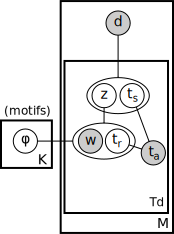
\includegraphics[width=0.38\textwidth]{PLSM}
\end{center}
 \vspace{-10pt}
 \caption{PLSM generative model: $d$ is the document variable, $z$ is the topic variable dependent on $d$ and $w$ is the word variable independent of $d$ given $z$. $d$ and $w$ are observed variables. $Td$ is the document length and $M$ is the number of documents}
\vspace{-10pt}
\end{wrapfigure}

Figure. \ref{fig:PLSM} shows the generative process of PLSM. Let $D = \{d_{1},d_{2},d_{3}, \cdots, d_{M}\}$ represent the set of documents (like videos from a surveillance camera), $W = \{w_{1},w_{2}, \cdots, w_{V}\}$ represents the vocabulary, $Ta = \{t_{1},t_{2}, \cdots, t_{Td}\}$ represents the time of occurrence of words in the document $d$. Then according to our model, the documents can be described by a set of motifs $Z=\{z_{1}, z_{2}, \cdots, z_{K}\}$ which have a duration of $Tz$ i.e $tr = \{t_{1}, t_{2}, \cdots, t_{Tz}\}$. Each motif can occur at any time $ts = \{t_{1}, t_{2}, \cdots, t_{Tds}\}$ in a document $d$. The generative process of the PLSM model can be described as follows:
\begin{itemize}

\item[$\cdot$] Pick a document $d$ from $P(d)$
\item[$\cdot$] Pick topic $z$ and it's starting time $ts$ from $P(z,ts|d)$
\item[$\cdot$] Pick a word $w$ and relative time $tr$ from $P(w,tr|z)$ 
\item[$\cdot$] Set ta=ts+tr or equivalently $P(ta|ts,tr)$ is a Dirac function at ta

\end{itemize}
The joint probability distribution $P(w,ta,d,z,ts,tr)$ can be obtained from the model as below:
\begin{eqnarray}
P(w,ta,d,z,ts,tr) & = & P(d)P(z,ts|d)P(w,tr|z)P(ta|tr,ts) \\
				 & = &\begin{cases}
    P(w,z,ts,tr,d),& \text{if } ta = ts+tr\\
    0,              & \text{otherwise}
\end{cases}
\end{eqnarray}

Given a corpus of documents $C$ in the form of term frequency matrix $n(w,ta,d)$, the liklihood of the data is given by the expression:
\begin{equation}
P(C) = \prod_{w,ta,d} P(w,ta,d)^{n(w,ta,d)}
\end{equation}

The motifs $P(w,tr|z)$ and their start times $P(z,ts|d)$ which form the parameters of the model can be infered from the observations. The inference is performed by maximizing the log-liklihood of the data. The inference is also guided towards estimating a sparse distribution of $P(z,ts|d)$ which is motivated in ~\cite{Varadarajan_IJCV_2012,varadarajan_probabilistic_2010}.
\begin{equation}
L(D|\theta) = \sum_{w,ts,tr,d} n(w,ts+tr,d)log(\sum_{z,ts} P(w,tr,d,z,ts)) + KL(U||P(z,ts|d))
\end{equation}
 Since the data is paratially observed, parameters are estimated using the expectation maximization algorithm.
 \begin{equation}
 E[L] = \sum_{w,ts,tr,z,d}n(w,ts+tr,d)P(z,ts|w,ts+tr,d)log(P(w,ts+tr,d,z,ts)) - \sum_{z,ts,d}\frac{\lambda_{d}}{K \cdot Tds} log(P(z,ts|d))
 \end{equation}
 
 The E-Step can be obtained Baye's rule
 \begin{equation}
 P(z,ts|w,ta,d) = \frac{P(z,ts|d)P(w,tr|z)}{\sum_{z,ts}P(z,ts|d)P(w,tr|z)}
 \end{equation}

The M-step expressions can be obtaiend by standard calculations
\begin{eqnarray}
P(z,ts|d) & \alpha & max(\epsilon, \sum_{w,tr}n(w,ts+tr,d)P(z,ts|w,ts+tr,d)- \frac{\alpha_{d}}{K\cdot Tds}) \\
P(w,tr|z) & \alpha & \sum_{ts,d}n(w,ts+tr,d)P(z,ts|w,ts+tr,d)
\end{eqnarray}

The term $\lambda_{d}$ as in ~\cite{Varadarajan_IJCV_2012,varadarajan_probabilistic_2010} is defined as $\lambda$$nd$ where nd is the number of words in the document $d$ and $\lambda$ indicates the sparsity level.